\chapter{Intalisasi}
	\section{Instalasi Python 3}
	Berikut adalah cara instalasi python 3 :
	\begin{enumerate}
	    \item Download python versi 3.7.4 
	    \item Run file download
	    \item Setelah itu akan muncul tampilan untuk instalasi
	    \par
	    \begin{figure}[!htbp]
	       \centering
		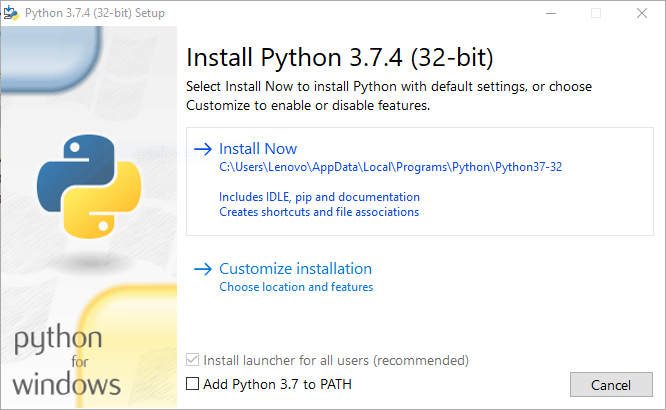
\includegraphics[width=8cm]{figures/1.PNG}
		\caption{Tampilan instalasi}
    	\end{figure}
    	
	    \item klik install now
	    \begin{figure}[!htbp]
	    	\centering
		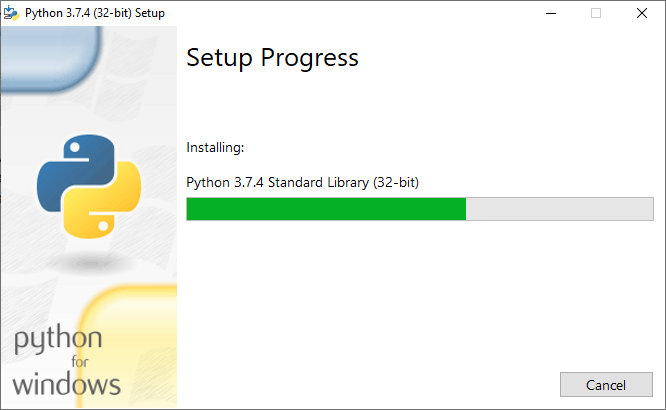
\includegraphics[width=8cm]{figures/2.PNG}
		\caption{Proses Intalasi}
    	\end{figure}
    	
    	\item proses instalasi akan di proses
	    \begin{figure}[!htbp]
		\centering
		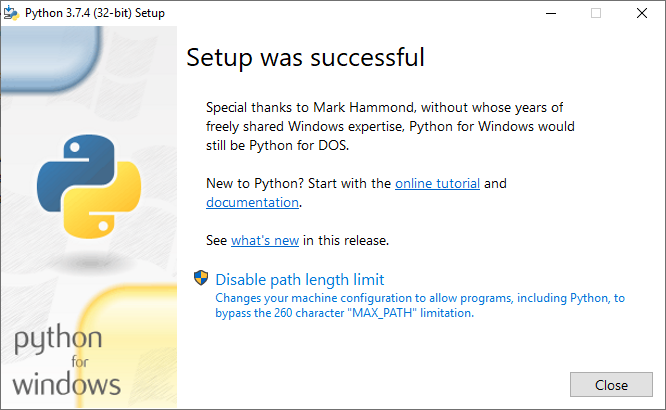
\includegraphics[width=8cm]{figures/3.PNG}
		\caption{Instalasi Sukses}
    	\end{figure}
	\end{enumerate}
	
	\newpage	
	\section{Instalasi Anaconda}
Berikut ini merupakan langkah-langkah cara instalasi Anaconda di windows:
\begin{enumerate}
	\item Pastikan kalian telah menginstall Python sebelumnya.
	\item Klik dua kali pada installer Anaconda. Installer anaconda bisa anda dapatkan di https://www.anaconda.com/distribution/
	\item Setelah itu akan muncul window installernya. Kemudian klik ''Next'' untuk memulai instalasi.
	\begin{figure}[!htbp]
		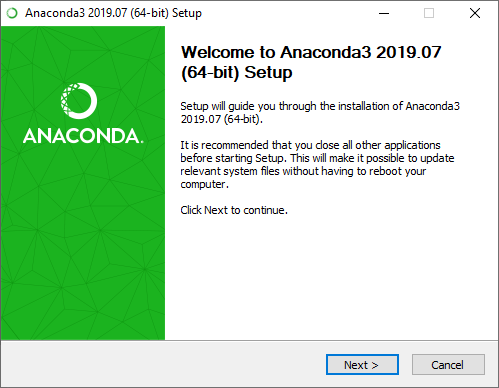
\includegraphics[width=8cm]{figures/anaconda.PNG}
		\centering
	\end{figure}
    \newpage
	\item Baca Lisensi Agreement Anacondanya. Lalu klik ''I Agree'' jika kalian menerimanya dan untuk melajutkannya instalasinya.
	\begin{figure}[!htbp]
		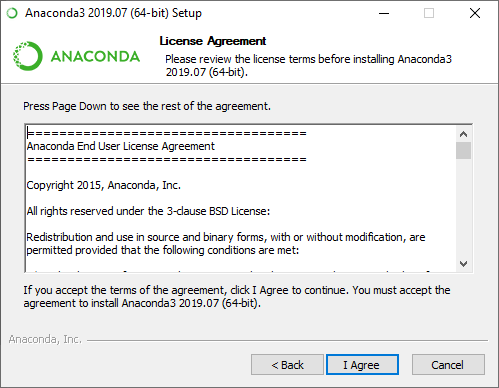
\includegraphics[width=8cm]{figures/anaconda1.PNG}
		\centering
	\end{figure}

	\item Selanjutnya diberi pilihan untuk menginstallnya, apakah hanya untuk kalian atau untuk semua pengguna. Pilih ''Just Me'', lalu klik ''Next''.
	\begin{figure}[!htbp]
	\centering
		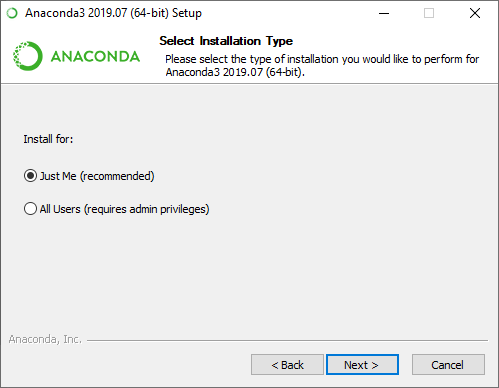
\includegraphics[width=8cm]{figures/anaconda2.PNG}
	\end{figure}
\newpage
	\item Kemudian pilih tujuan instalasinya. Disini saya biarkan default folder instalasinya. Setelah itu, klik ''Next''.
	\begin{figure}[!htbp]
		\centering
		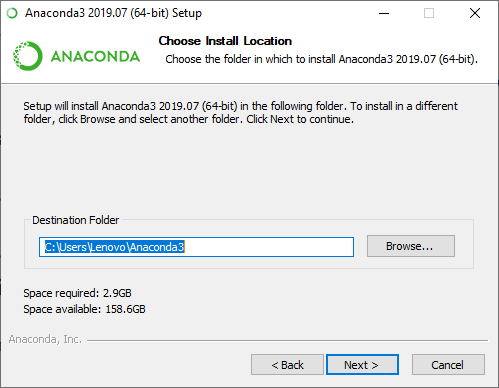
\includegraphics[width=8cm]{figures/anaconda3.PNG}
	\end{figure}

	\item Setelah itu, kalian diberi beberapa opsi tambahan. Opsi pertama yaitu, ''Add Anaconda to my PATH environment variable''. Opsi ini akan menambahkan Anaconda ke PATH sistem environment variable. Opsi kedua yaitu, ''Register Anaconda as my default Python 3.7''. Opsi ini akan mendaftarkan Anaconda sebagai system Python 3.7. Saya centang kedua opsi tersebut, lalu klik ''Install''.
	\begin{figure}[!htbp]
		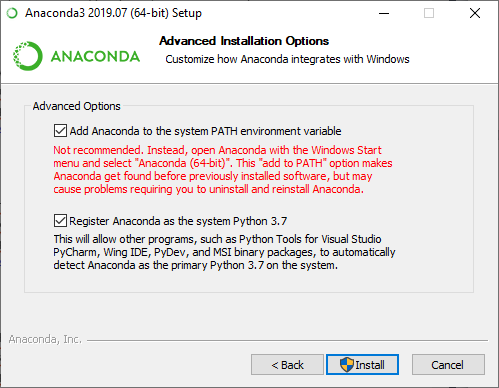
\includegraphics[width=8cm]{figures/Anaconda4.PNG}
		\centering
	\end{figure}
\newpage
	\item Tunggu hingga proses instalasi selesai.
	\begin{figure}[!htbp]
		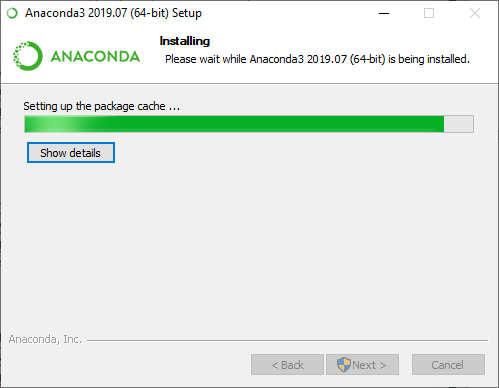
\includegraphics[width=8cm]{figures/anaconda5.PNG}
		\centering
	\end{figure}

	\item Kemudian klik ''Next'' untuk melanjutkan.
	\begin{figure}[!htbp]
		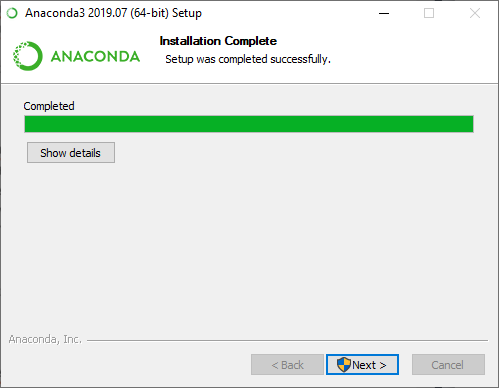
\includegraphics[width=8cm]{figures/ana6.PNG}
		\centering
	\end{figure}
\newpage
	\item Selanjutnya klik next untuk melanjutkan
	\begin{figure}[!htbp]
		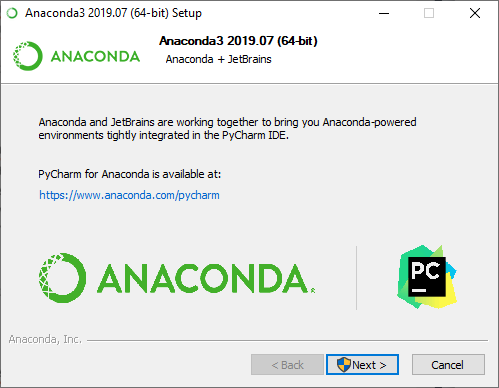
\includegraphics[width=8cm]{figures/ana7.PNG}
		\centering
	\end{figure}

	\item Kemudian klik ''Finish'' untuk menyelesaikan.
	\begin{figure}[!htbp]
		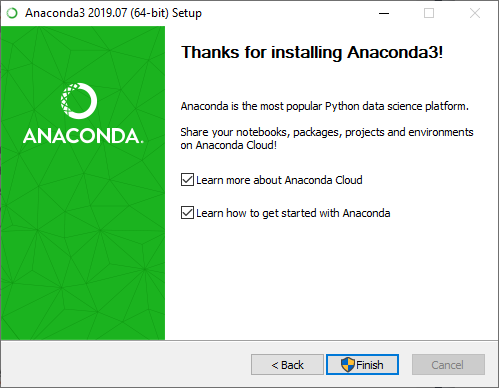
\includegraphics[width=8cm]{figures/ana8.PNG}
		\centering
	\end{figure}
\newpage
	\item Untuk mengecek apakah Anaconda telah terinstall yaitu dengan cara membuka Command Prompt. Lalu ketikan ''conda -V'' dan tekan enter, kode itu akan mengecek versi Anaconda yang terinstall.
	\begin{figure}[!htbp]
		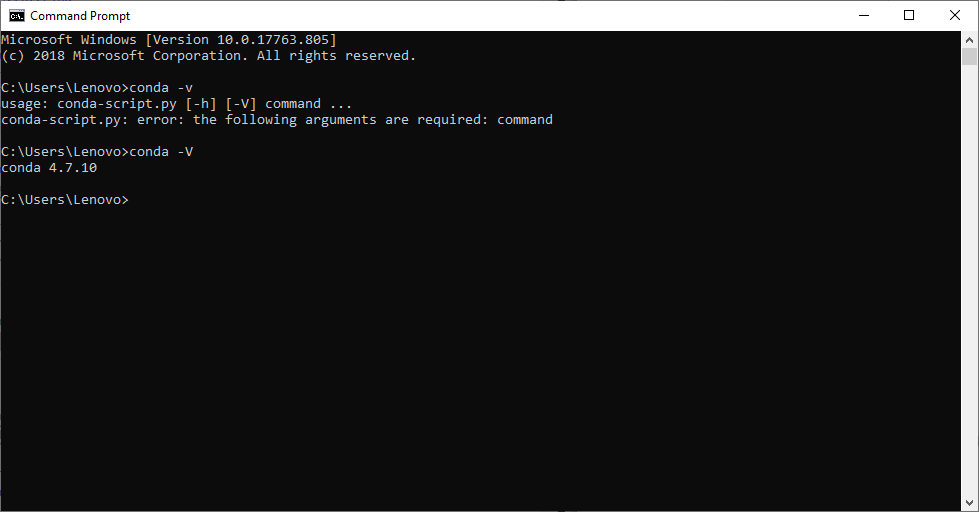
\includegraphics[width=10cm]{figures/akhirconda.PNG}
		\centering
	\end{figure}

\end{enumerate}

\section{Penggunaan Spyder}

Terdapat 2 cara menjalankan Spyder. Yang pertama dengan Anaconda Prompt dan yang kedua dengan Anaconda Navigation. Berikut ini merupakan langkah-langkah cara menjalankan Spyder pada anconda prompt:

\begin{itemize}
	\item Anaconda Prompt
	\begin{enumerate}
		
		\item Pertama klik start, lalu cari ''Anaconda Prompt''.
		\item Selanjutnya akan muncul sebuah prompt. Kemudian ketikan ''start spyder'' dan tekan enter.
		\begin{figure}[!htbp]
			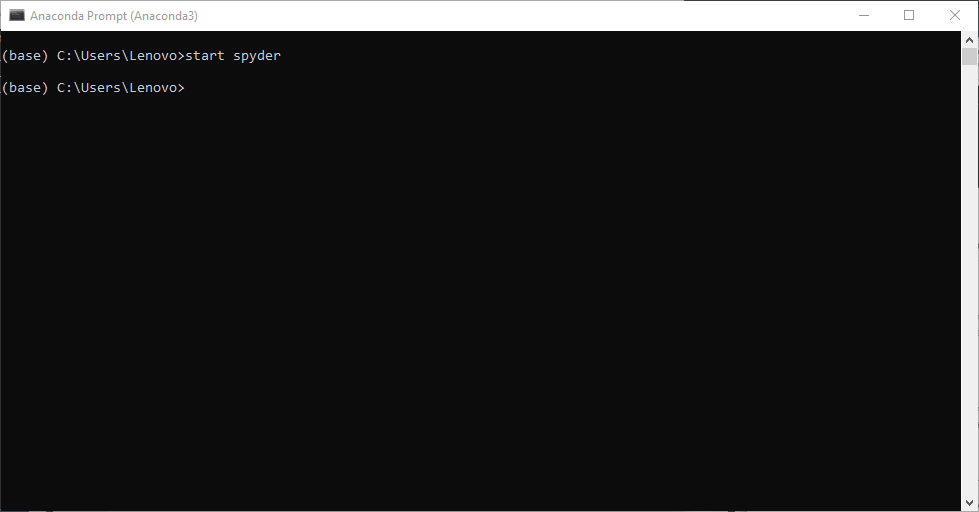
\includegraphics[width=8cm]{figures/spy1.PNG}
			\centering
			\caption{Ketikan Start Spyder}
		\end{figure}
		
		\newpage
		\item Lalu tunggu sampai selesai.
		\begin{figure}[!htpb]
			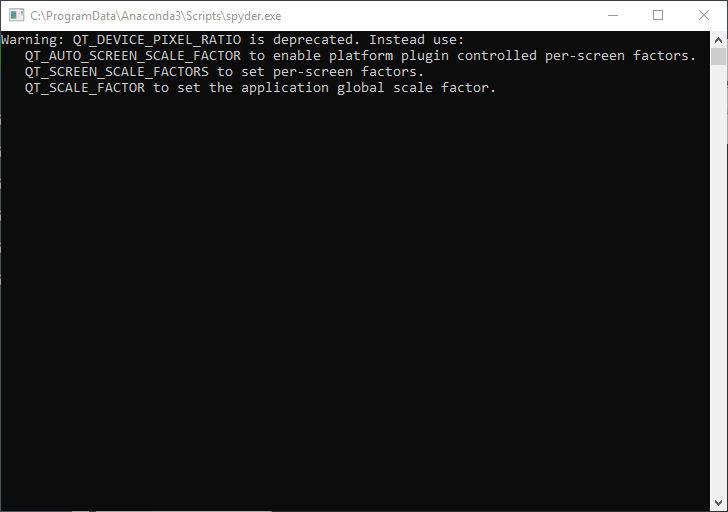
\includegraphics[width=8cm]{figures/spy2.PNG}
			\centering
			\caption{Proses}
		\end{figure}
		
		\item Spyder akan terbuka
		\begin{figure}[!htbp]
			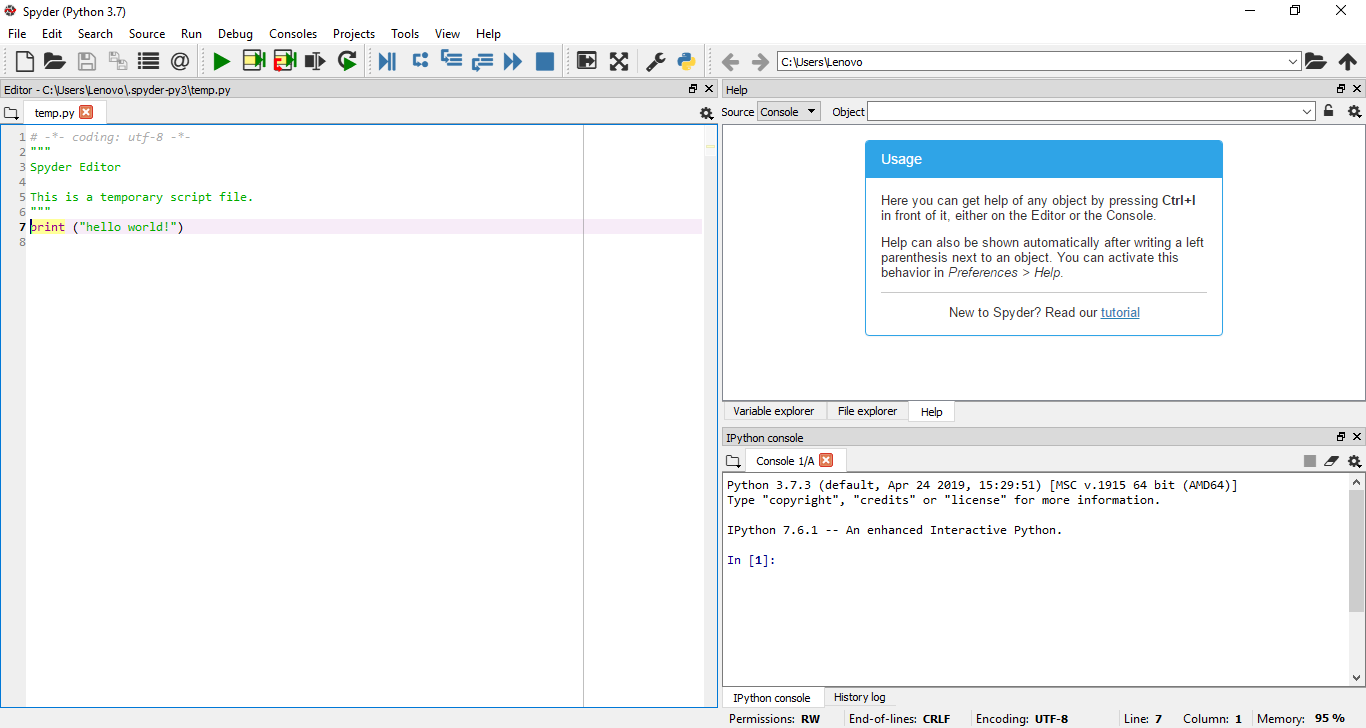
\includegraphics[width=8cm]{figures/spy3.PNG}
			\centering
			\caption{Spyder}
		\end{figure}
	\end{enumerate}
\end{itemize}
\newpage

\section {Instalasi PIP}
\begin{enumerate}
    \item Unduh get-pip.py ke folder di komputer Anda.
    \item Buka prompt perintah dan navigasikan ke folder yang berisi get-pip.py.
    \item Jalankan perintah berikut "Python get-pip.py
		\begin{figure}[!htpb]
			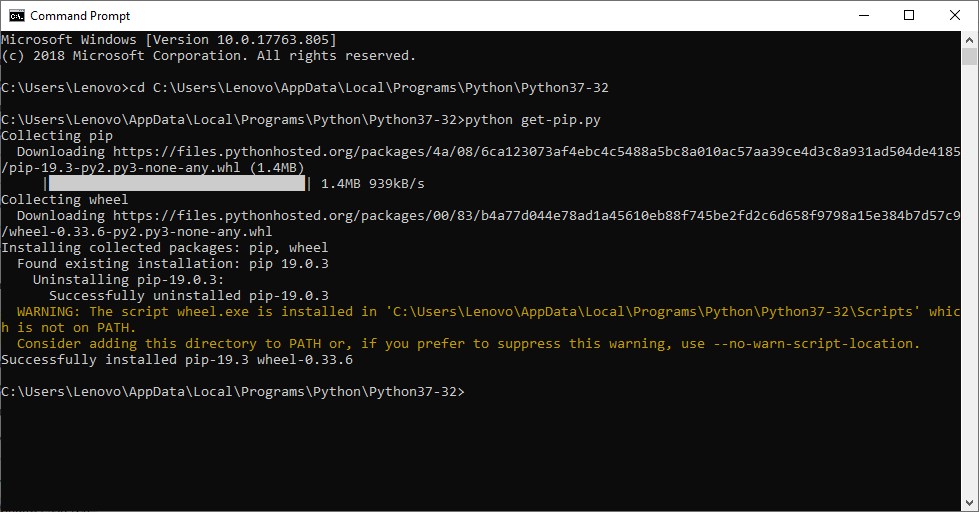
\includegraphics[width=8cm]{figures/4.PNG}
			\centering
			\caption{Instalasi PIP}
		\end{figure}
\end{enumerate}

\section {Cara Setting Environment}
\begin{enumerate}
    \item Pertama yaitu Python 3.7.4 sudah diinstall
    \item Masuk ke system pada Control Panel Control "Panel/System and Security/System"
    \begin{figure}[!htpb]
			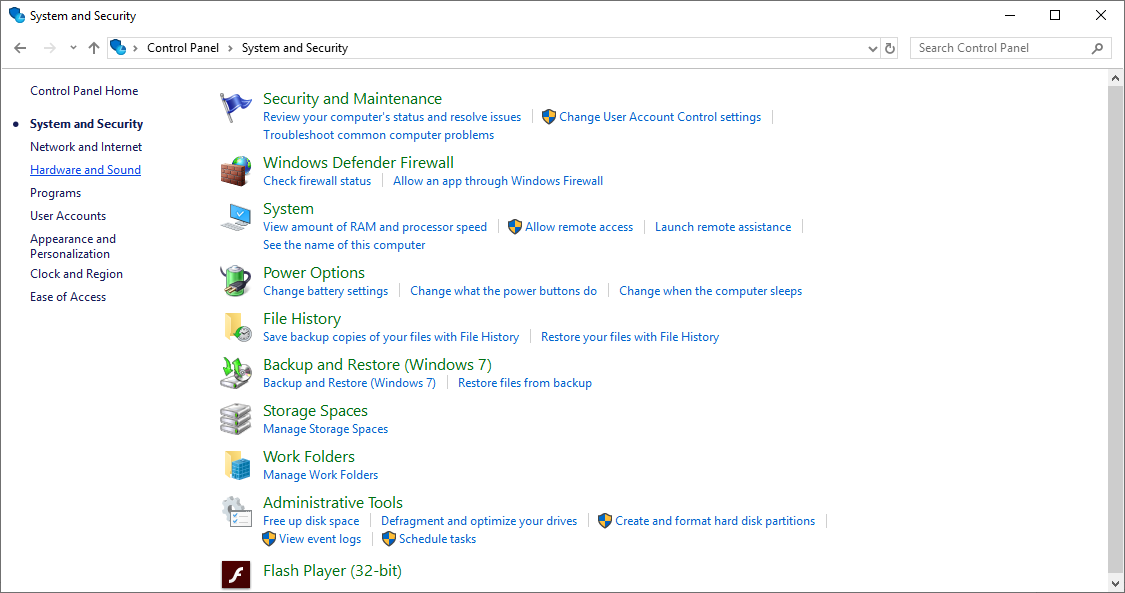
\includegraphics[width=8cm]{figures/6.PNG}
			\centering
			\caption{Masuk ke kontrol panel}
		\end{figure}
    \item Kemudian klik “Advanced system settings“
		\begin{figure}[!htpb]
			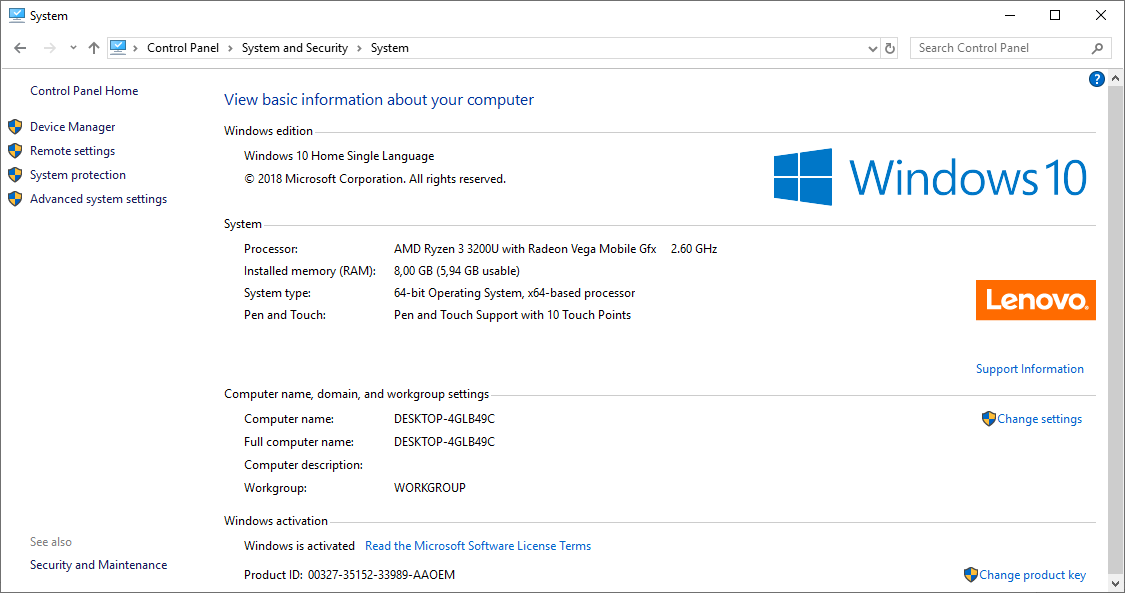
\includegraphics[width=8cm]{figures/7.PNG}
			\centering
			\caption{Klik andvance system settings}
		\end{figure}
		\newpage
	\item  Lanjut klik “Environment Variables” maka akan muncul lagi “Environment Variables”
    \begin{figure}[!htpb]
			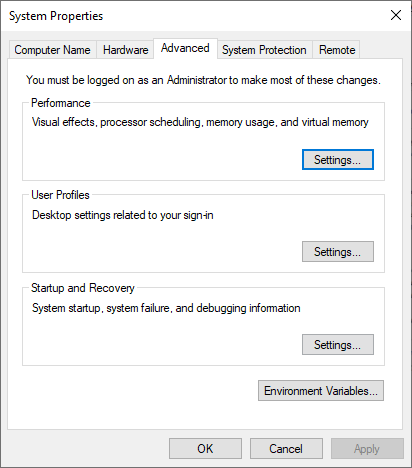
\includegraphics[width=8cm]{figures/8.PNG}
			\centering
			\caption{Klik Environmet Variabeles}
		\end{figure}
		\newpage
    \item Pada bagian System variables, scroll sampai ketemu Path. (Path adalah nama Variable)
		\begin{figure}[!htpb]
			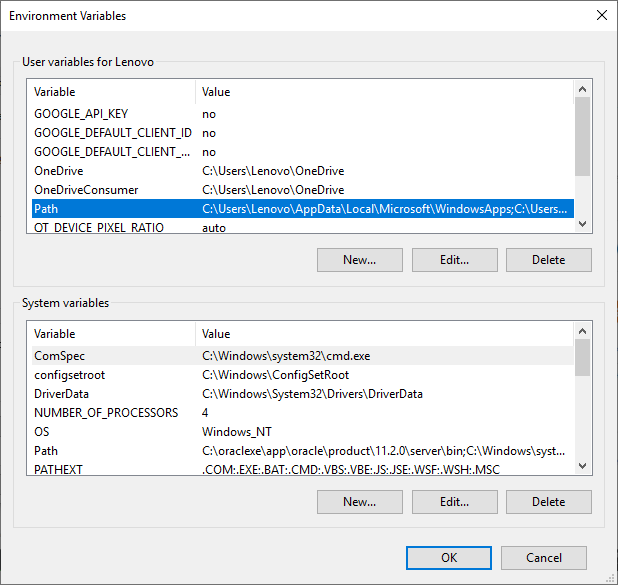
\includegraphics[width=8cm]{figures/sembil.PNG}
			\centering
			\caption{Scroll path}
		\end{figure}
			
	\item klik Path akan muncul tampilan Environment Variables. 
		\begin{figure}[!htpb]
			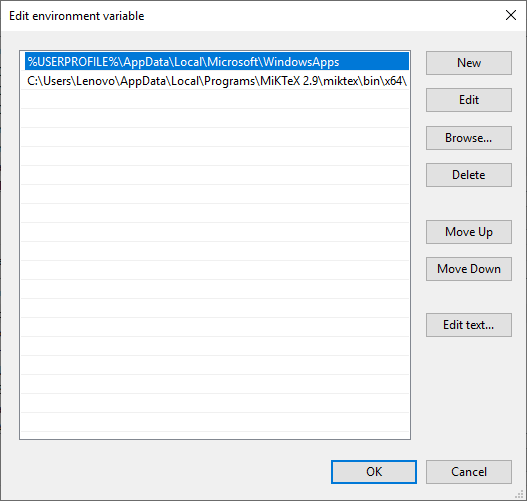
\includegraphics[width=8cm]{figures/10.PNG}
			\centering
			\caption{Klik Path}
		\end{figure}
	\newpage
	\item Lalu klik New tambahkan path sesuai versi python yang diinstall
		\begin{figure}[!htpb]
			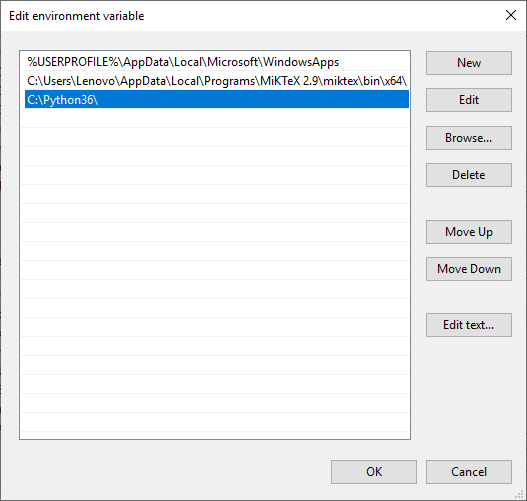
\includegraphics[width=8cm]{figures/11.PNG}
			\centering
			\caption{New Path}
		\end{figure}
\end{enumerate}
\section{Mencoba entrepreter/cli melakui terminal atau cmd windows}
    \begin{enumerate}
        \item Buka Command Prompt
        \item Ketik "Python" lalu enter
        \begin{figure}[!htpb]
			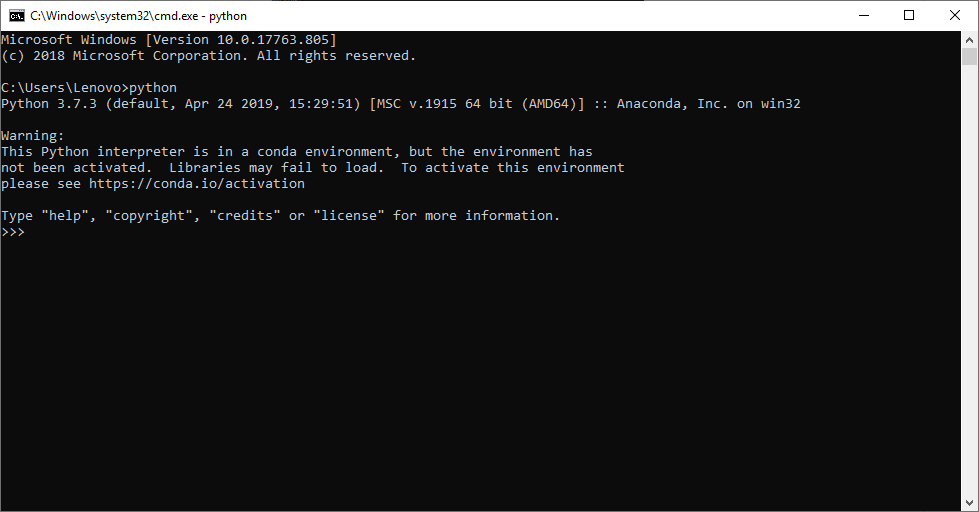
\includegraphics[width=10cm]{figures/envinew.PNG}
				\centering
			\caption{Ketik Python}
		\end{figure}
		\newpage
        \item Lalu ketik exit() lalu enter
        \begin{figure}[!htpb]
			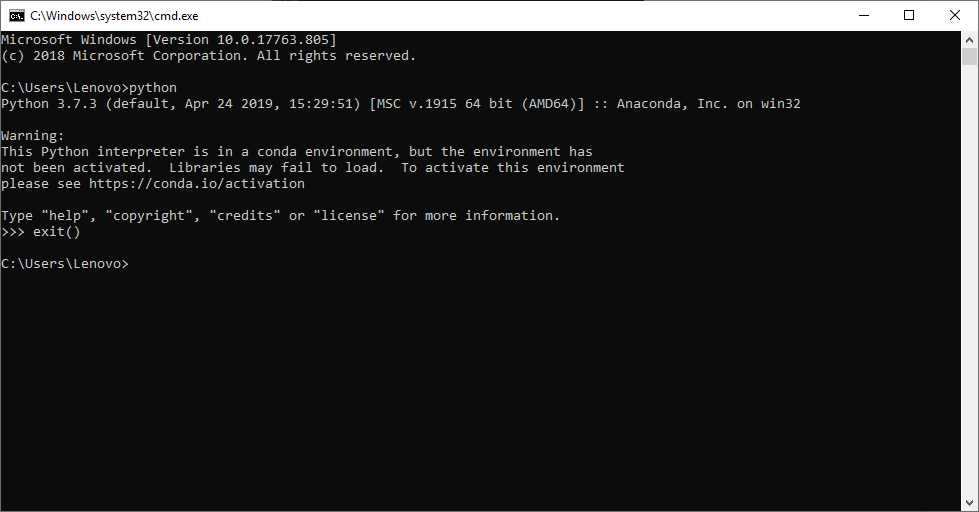
\includegraphics[width=10cm]{figures/envi2.PNG}
				\centering
			\caption{tampilan setelah exit}
		\end{figure}
		\item lalu ketik conda activate, lalu enter
		\begin{figure}[!htpb]
			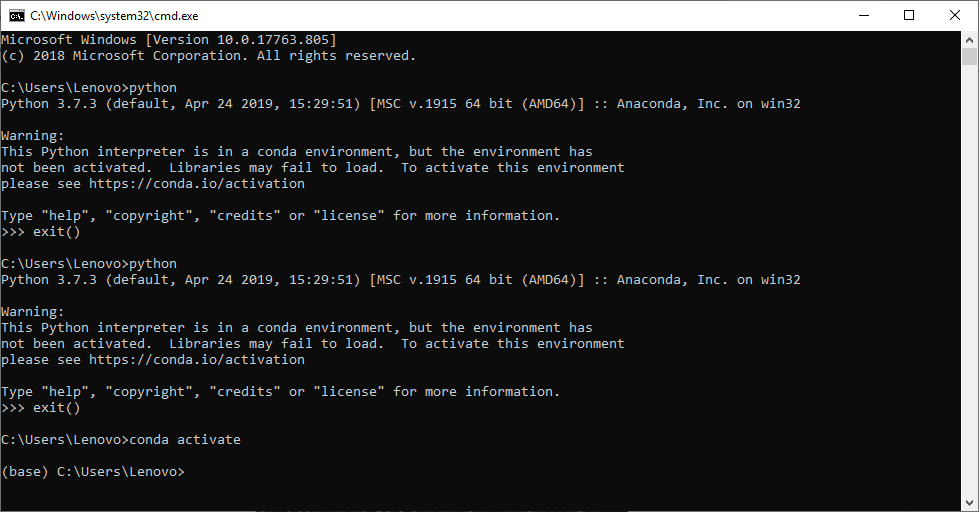
\includegraphics[width=10cm]{figures/envi3.PNG}
				\centering
			\caption{tampilan setelah conda activate}
		\end{figure}
		\newpage
		\item Lalu ketik kembali python lalu enter
		\begin{figure}[!htpb]
			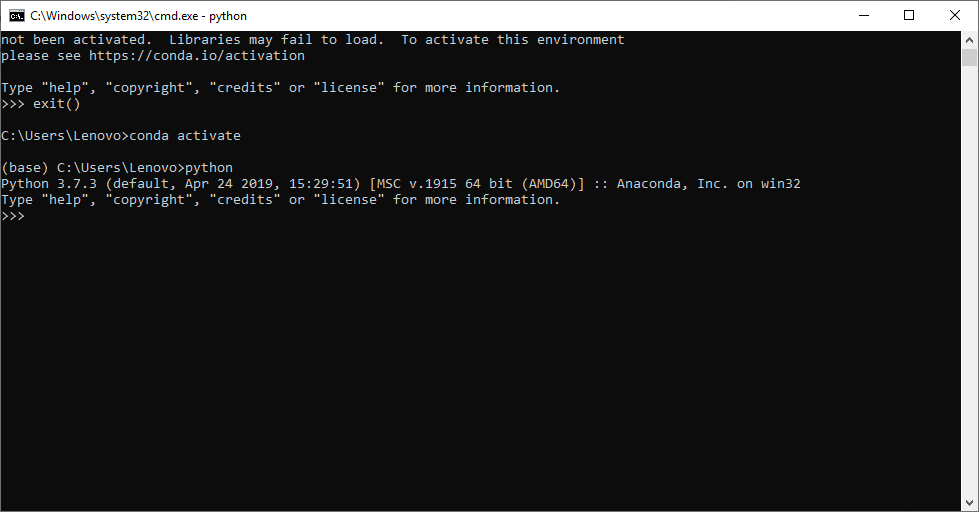
\includegraphics[width=10cm]{figures/envi4.PNG}
				\centering
			\caption{Ketik kembali Python}
		\end{figure}
        \item Lalu buat print ("Hello Wolrd!") Lalu enter.
        \item Maka akan ditampilkan Hello world dari hasil print diatas
        \begin{figure}[!htpb]
			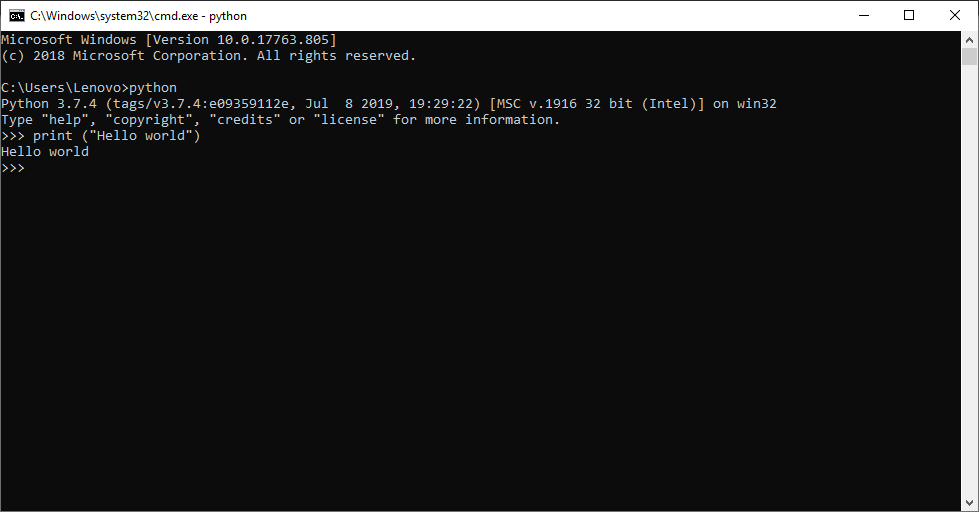
\includegraphics[width=10cm]{figures/interpreter.PNG}
				\centering
			\caption{Enterpreter/cli melalui CMD}
		\end{figure}
    \end{enumerate}
    
    \newpage
    \section{Menjalankan dan mengupdate anaconda dan spyder}
    Berikut adalah cara untuk menjalankan dan mengupdate anaconda dan spyder dapat menggunakan cmd dan anaconda prompt:
    \begin{enumerate}
        \item Buka CMD, Lalu ketik Python dan enter
        \item Lalu ketik exit ()
        \item Ketik conda activate lalu enter
        \item untuk melakukan update pada anaconda ketik " conda install -c anaconda python "
        \begin{figure}[!htpb]
			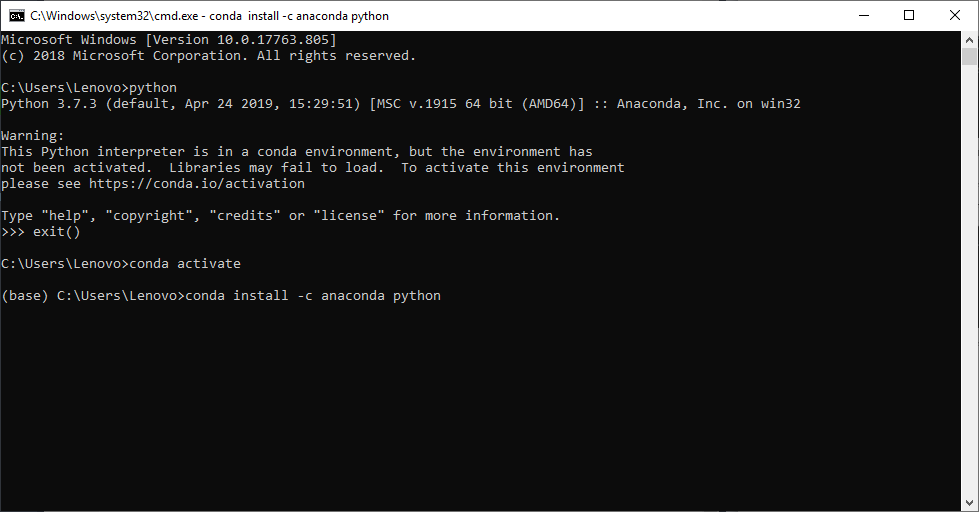
\includegraphics[width=8cm]{figures/up.PNG}
			\centering
			\caption{ketik perintah untuk update}
		\end{figure}
        \item lalu akan muncul perintah apakah anda yakin untuk melakukan update atau tidak (Y/N)?
        \begin{figure}[!htpb]
			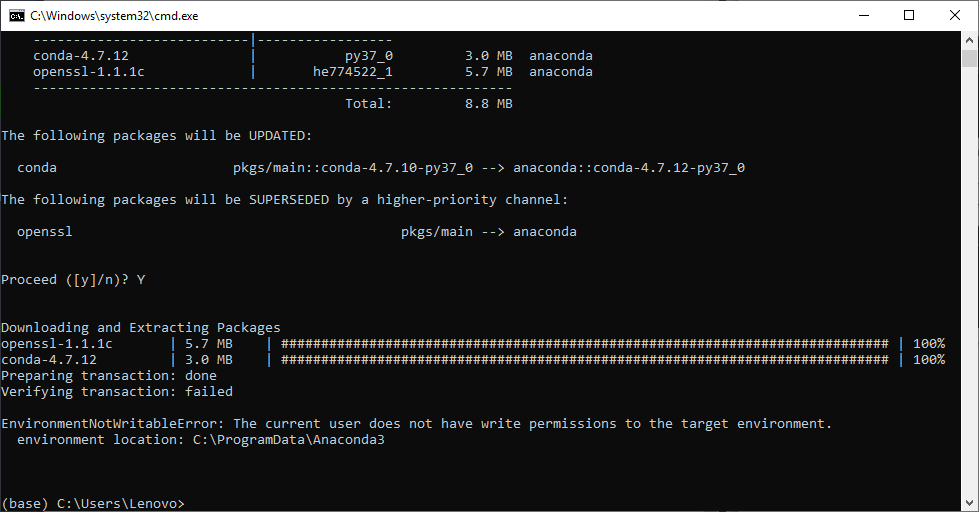
\includegraphics[width=8cm]{figures/upfinish.PNG}
			\centering
			\caption{Update Anaconda dan Spyder selesai}
		\end{figure}
        
    \end{enumerate}
    \section{Menjalankan Script Hello World pada spyder}
     \begin{enumerate}
        \item Buka Spyder
        \item Ketik kodingan print ("Hello Wolrd!").
        \item Lalu klik compile/run
        \item Setelah itu akan muncul hasil print hello world pada console.
        \begin{figure}[!htpb]
			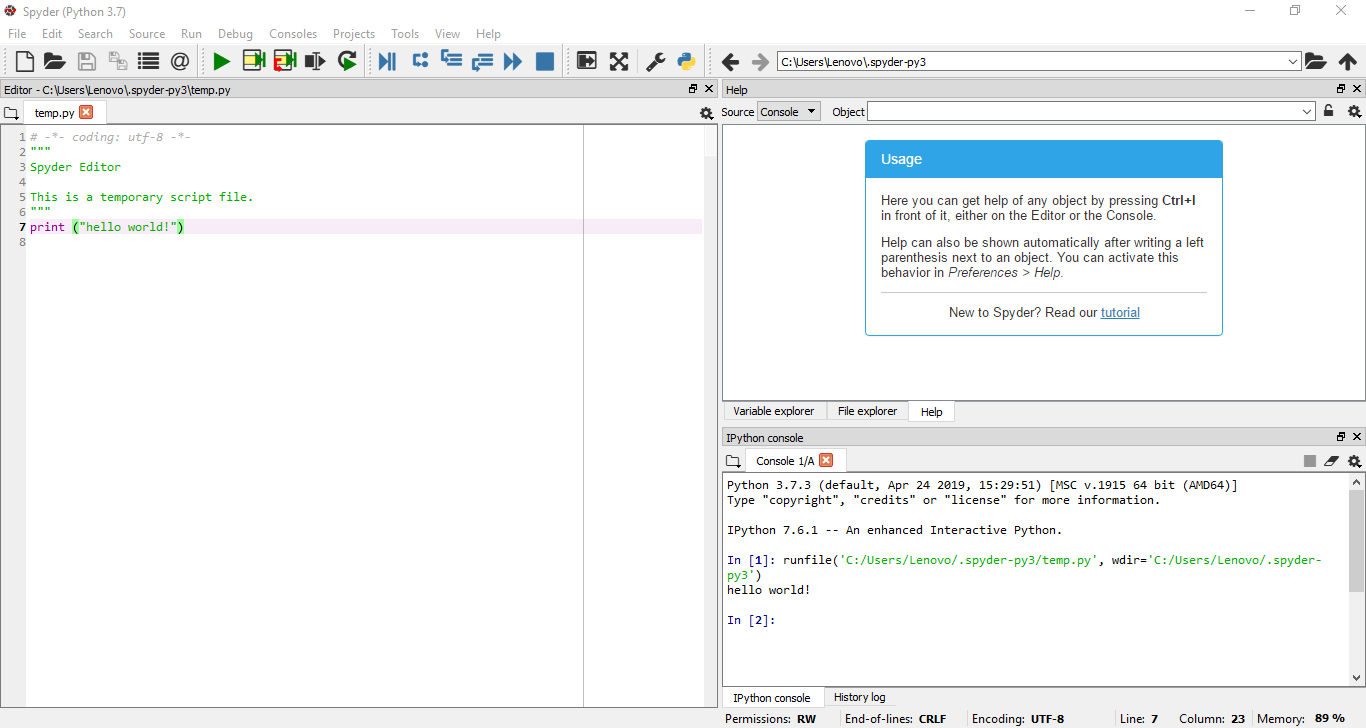
\includegraphics[width=10cm]{figures/printhello.PNG}
			\centering
			\caption{Hello World pada Spyder}
		\end{figure}
    \end{enumerate}
    
    \newpage
    
    \section{Cara menjalankan Script otomatis login aplikasi akademik dengan library selenium dan inputan user}
    \begin{enumerate}
        \item Yang pertama yaitu buka CMD, Lalu lakukan instalasi Selenium dengan mengetik "pip install selenium" secara langsung melalui command prompt.
        \begin{figure}[!htpb]
			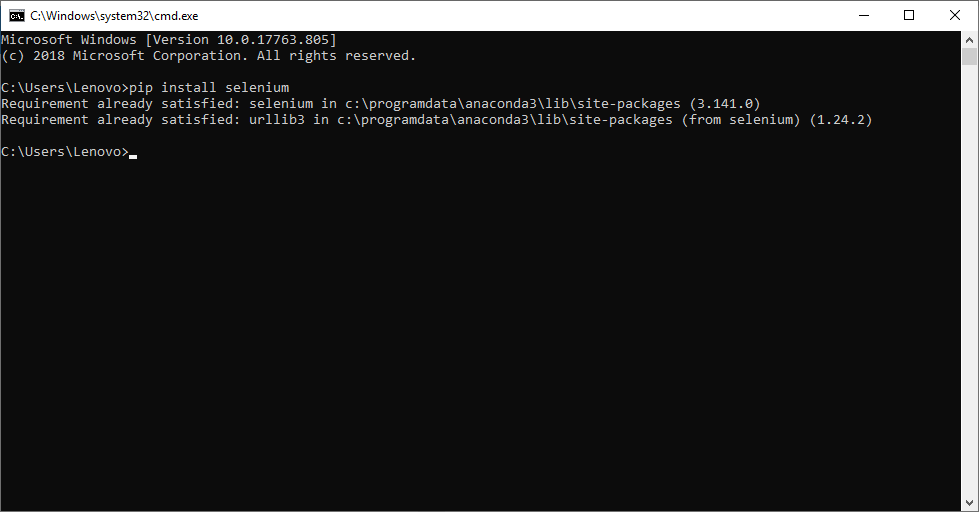
\includegraphics[width=10cm]{figures/selenium.PNG}
			\centering
			\caption{Install Selenium di Command Prompt}
		\end{figure}
		\item Yang kedua yaitu download geckoddriver.exe sesuai versi yang anda butuhkan.
		\item tambahkan file geckoddriver.exe ke dalam system32 pada local disk data C:
		\begin{figure}[!htpb]
			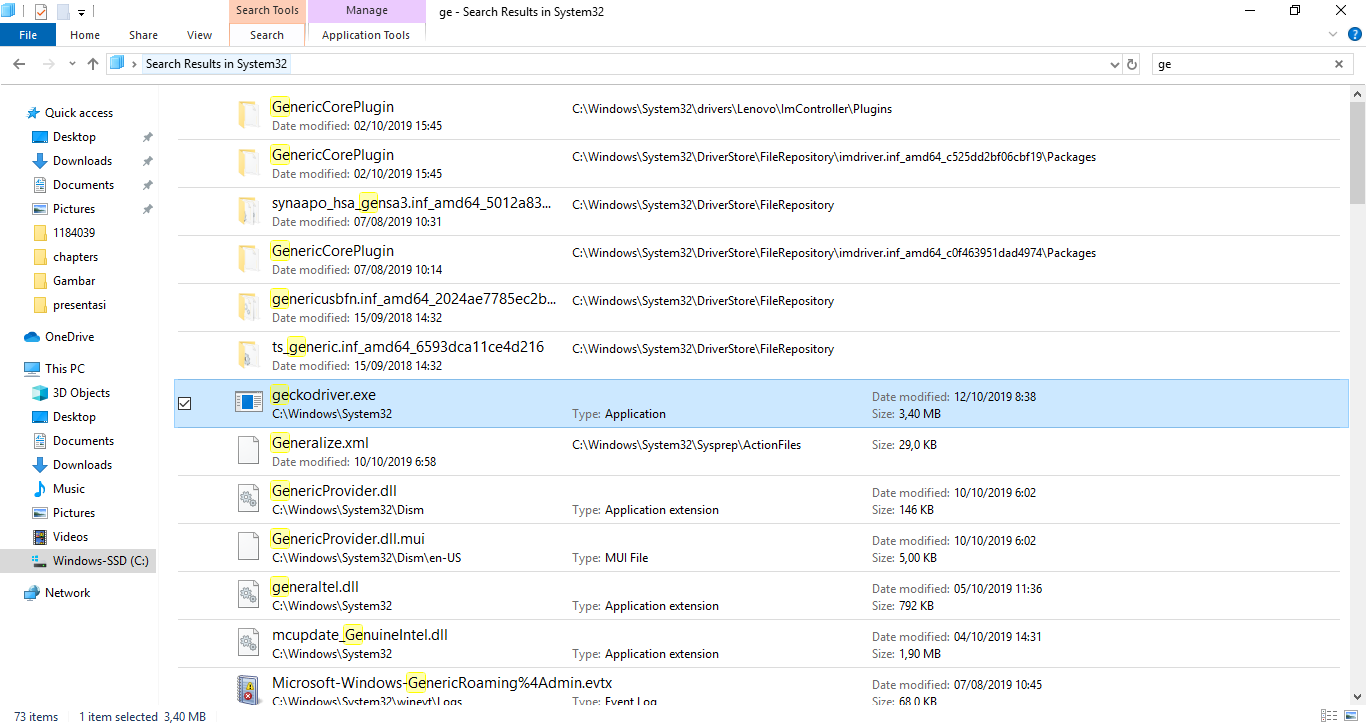
\includegraphics[width=10cm]{figures/sellgock.PNG}
			\centering
			\caption{Tambahkan geckodriver.exe kedalam local disk C}
		\end{figure}
		\item Buka Spyder untuk membuat codingannya. Buat file kodingan lalu save 
		\item Ketik kodingan selenium yang akan dijalankan dan sesuai dengan browser yang digunakan, seperti yg saya gunakan yaitu chrome.
		\begin{figure}[!htpb]
			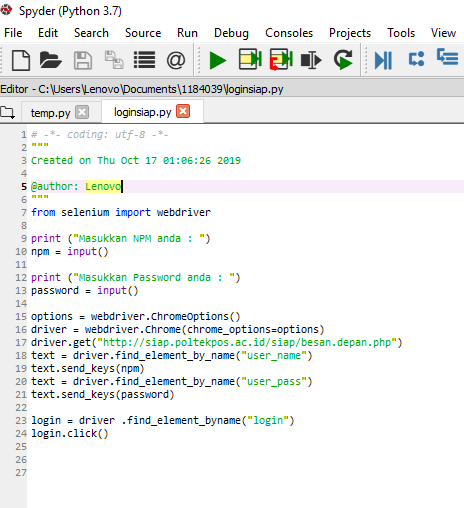
\includegraphics[width=5cm]{figures/sellkoding.png}
			\centering
			\caption{Kodingan pada Chrome}
		\end{figure}
		\item Setelajh programnya dijalankan maka otomatis akan langsung login ke website siap politeknik pos indonesia
		\begin{figure}[!htpb]
			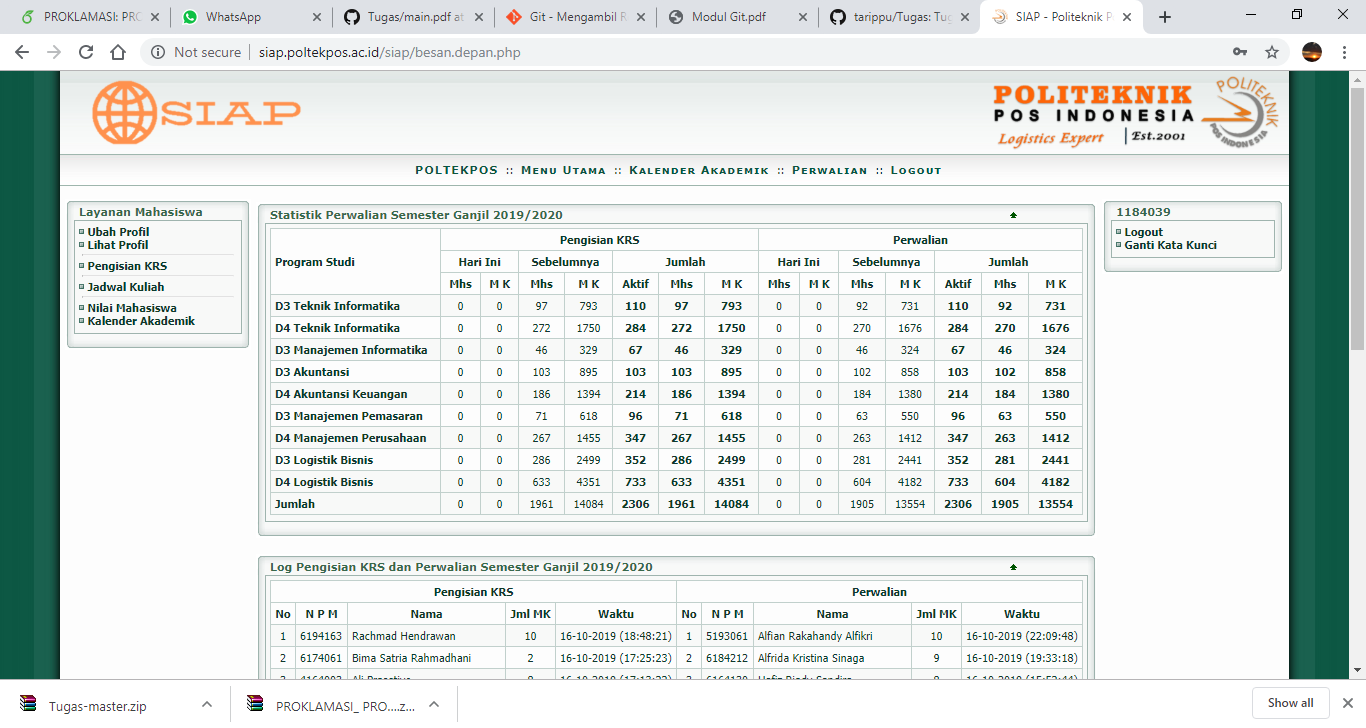
\includegraphics[width=10cm]{figures/siap.PNG}
			\centering
			\caption{Login ke website SIAP}
		\end{figure}
    \end{enumerate}

    
    \newpage
    
    \section{Cara pemakaian variable explorer di spyder}
    \begin{enumerate}
        \item Buka Spyder
        \item Ketik kodingan hello = "sayang kamu" 
        \item Lalu buat print "hello"
        \item Lalu klik compile/run
        \item Setelah itu akan muncul hasil print hello world pada console.
        \item Klik Variabel explorer pada pojok kanan
        \item Maka akan muncul tab variabel explorer diatas console.
        \begin{figure}[!htpb]
			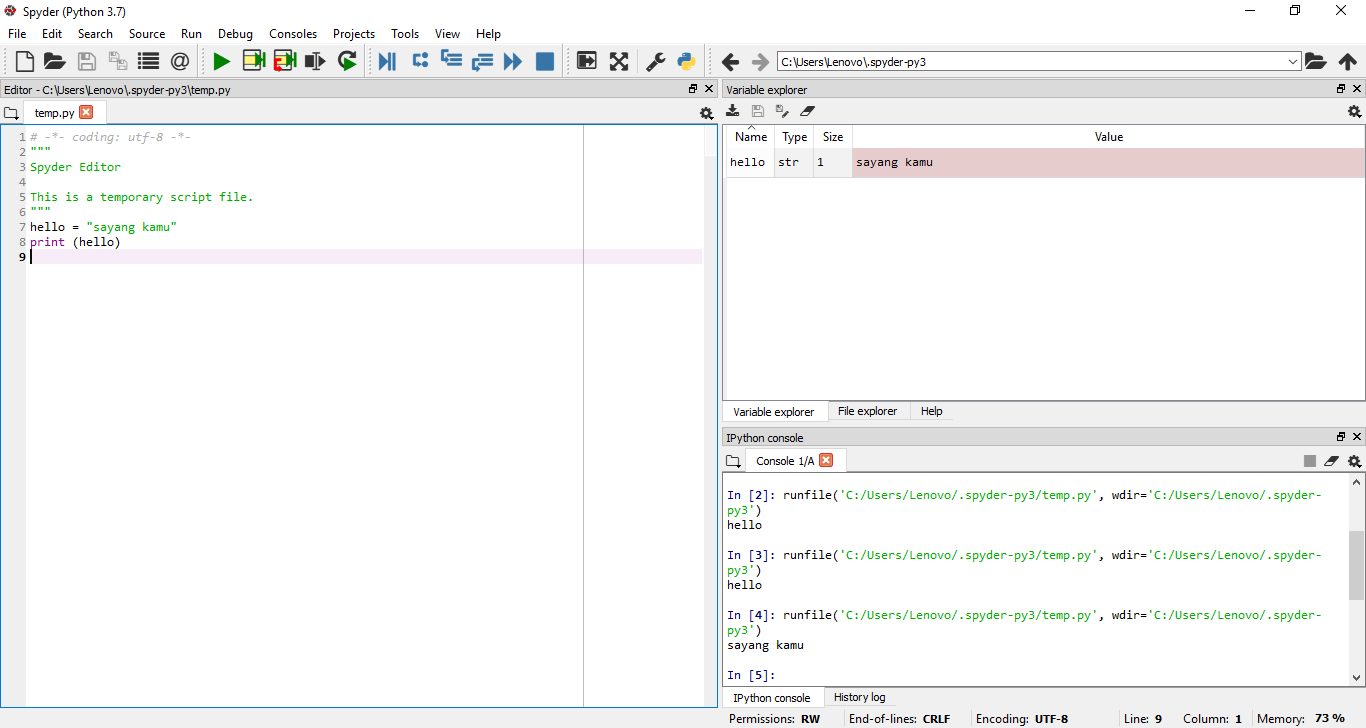
\includegraphics[width=10cm]{figures/variable.PNG}
				\centering
			\caption{Variabel explorer}
		\end{figure}
    \end{enumerate}
    
    
    